% id: 119-92
% book: 쎈B 공통수학1 · 09 순열과 조합
% section: 유형 24 평행사변형의 개수
% figure: tikz:fig-119-92
% answer: 
% answer_source: 
% variant_level: 0 (원본 전사)
% 이 파일은 build.mjs 가 items.json 에서 만든다. 고칠 때는 items.json 을 고친다.
\smash{\raisebox{1.5mm}{\dmkichul{쎈B 공통수학1 119쪽 92번}}}
\noindent\begin{minipage}[t]{0.58\linewidth}\vspace{0pt}\raggedright 오른쪽 그림과 같이 3개, 4개, 4개의 평행한 직선이 서로 만날 때, 이 평행한 직선으로 만들어지는 평행사변형의 개수를 구하시오.\end{minipage}\hfill\begin{minipage}[t]{0.4\linewidth}\vspace{0pt}\centering \resizebox{\ifdim\width>\linewidth\linewidth\else\width\fi}{!}{% 119-92(119쪽) — 세 방향의 평행한 직선 3개·4개·4개가 서로 만나는 그림. 스캔 화질이 낮아 TikZ 로 다시 그림.
% 원문 그대로 가로 방향 4개 · 오른쪽 위로 기운 것 4개 · 오른쪽 아래로 기운 것 3개. 라벨·표시는 원문에 없다.
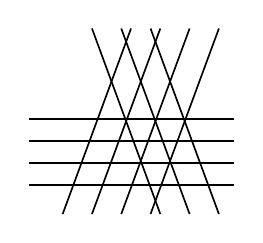
\begin{tikzpicture}[scale=0.62, line width=0.6pt]
  \foreach \y in {0,0.45,0.9,1.35} { \draw (-0.3,\y) -- (3.9,\y); }
  \foreach \a in {0.4,1.0,1.6,2.2} { \draw (\a,-0.6) -- (\a+1.4,3.2); }
  \foreach \b in {1.0,1.6,2.2} { \draw (\b,3.2) -- (\b+1.4,-0.6); }
\end{tikzpicture}
}\end{minipage}\par
